% Session 5 -- the Kitaev chain: which Majoranas pair with which.
% Placement: sec. "The Kitaev chain", after the SSH-recognition paragraph.
% Rendered by figures/blender/s05f05_kitaev.py, labels in figures/overlays/s05f05_kitaev.tex.
\begin{aqmfigure}{fig:s05:kitaev}{The Kitaev chain in terms of Majorana variables, for $N=5$ sites
(so $\gamma_{2N}=\gamma_{10}$), seen from above. Each site carries two balls, its two Majorana
halves, and a translucent capsule binds two halves together. Splitting every electron into its two
Majorana halves (5.17) has no physical content by itself, and what matters is which halves the
Hamiltonian binds together. In the trivial phase, at the top, the binding is inside each site. The
two halves of each electron stay bound to each other, as they were in the vacuum, and every mode
costs energy. In the topological phase, at the bottom, the binding is between sites, $\gamma_{2n}$
with $\gamma_{2n+1}$, and the pattern has one bond missing at each end. So $\gamma_1$ and
$\gamma_{2N}$ do not appear in (5.21), cost no energy and are at opposite ends of the sample. The
ordinary fermion that they would form together has been split into two halves, which are now
separated by the length of the chain, and this is what \emph{deconfined} means here. This is the
fully dimerized SSH chain of the topological-band-structure session with its two remaining end
sites, with new labels, so the counting is the same and only the operators are new.}
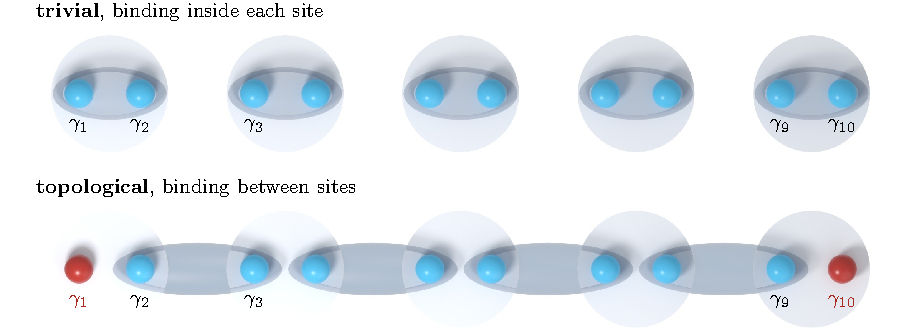
\includegraphics{figures/pdf/s05f05_kitaev.pdf}
\end{aqmfigure}
